\documentclass[a4paper]{exam}

\usepackage{amsmath,amssymb, amsthm}
\usepackage{geometry}
\usepackage{graphicx}
\usepackage{hyperref}
\usepackage{titling}
\usepackage{tikz}
\usepackage{tikz-qtree}
\usepackage{framed}

% \graphicspath{{images/}}


\newtheorem{definition}{Definition}
\newtheorem{theorem}{Theorem}
\newtheorem{corollary}{Corollary}
\newtheorem{axiom}{Axiom}
\theoremstyle{claim}
\newtheorem{claim}{Claim}

% Header and footer.
\pagestyle{headandfoot}
\runningheadrule
\runningfootrule
\runningheader{CS/MATH 113 2025}{Pset 10: Graph}{\theauthor}
\runningfooter{}{Page \thepage\ of \numpages}{}
\firstpageheader{}{}{}

% \printanswers %Uncomment this line

\title{Problem Set 10: Graph}
\author{Blingblong} % <=== replace with your student ID, e.g. xy012345
\date{CS/MATH 113 Discrete Mathematics\\Habib University\\Spring 2025}


% \qformat{{\large\bf \thequestion. \thequestiontitle}\hfill}
% \boxedpoints


\begin{document}
\maketitle      


\section*{Problems}
In the following problem set assume all the graphs are simple and finite unless specified otherwise.
\begin{questions}
  \question In parkour civilization everything is parkour. For some positive integer $m$ there are at most $2m+1$ houses at the parkour pro level of parkour civilization. From each house you can parkour to exactly $m$ other houses. Every parkour pro is sleeping inside a house. Tung Tung Tung Sahur wants to wake up all the parkour pros. For this he wishes to parkour to each of the houses in parkour civilization. By the help of Agent 5.5 he can teleport to any one house of his choice by then from there he would have to parkour to every other house he wishes to visit. Can Tung Tung Tung Sahur visit every house and wake up every parkour pro? Give a formal proof for your answer.
  \begin{figure}[h!]
    \centerline{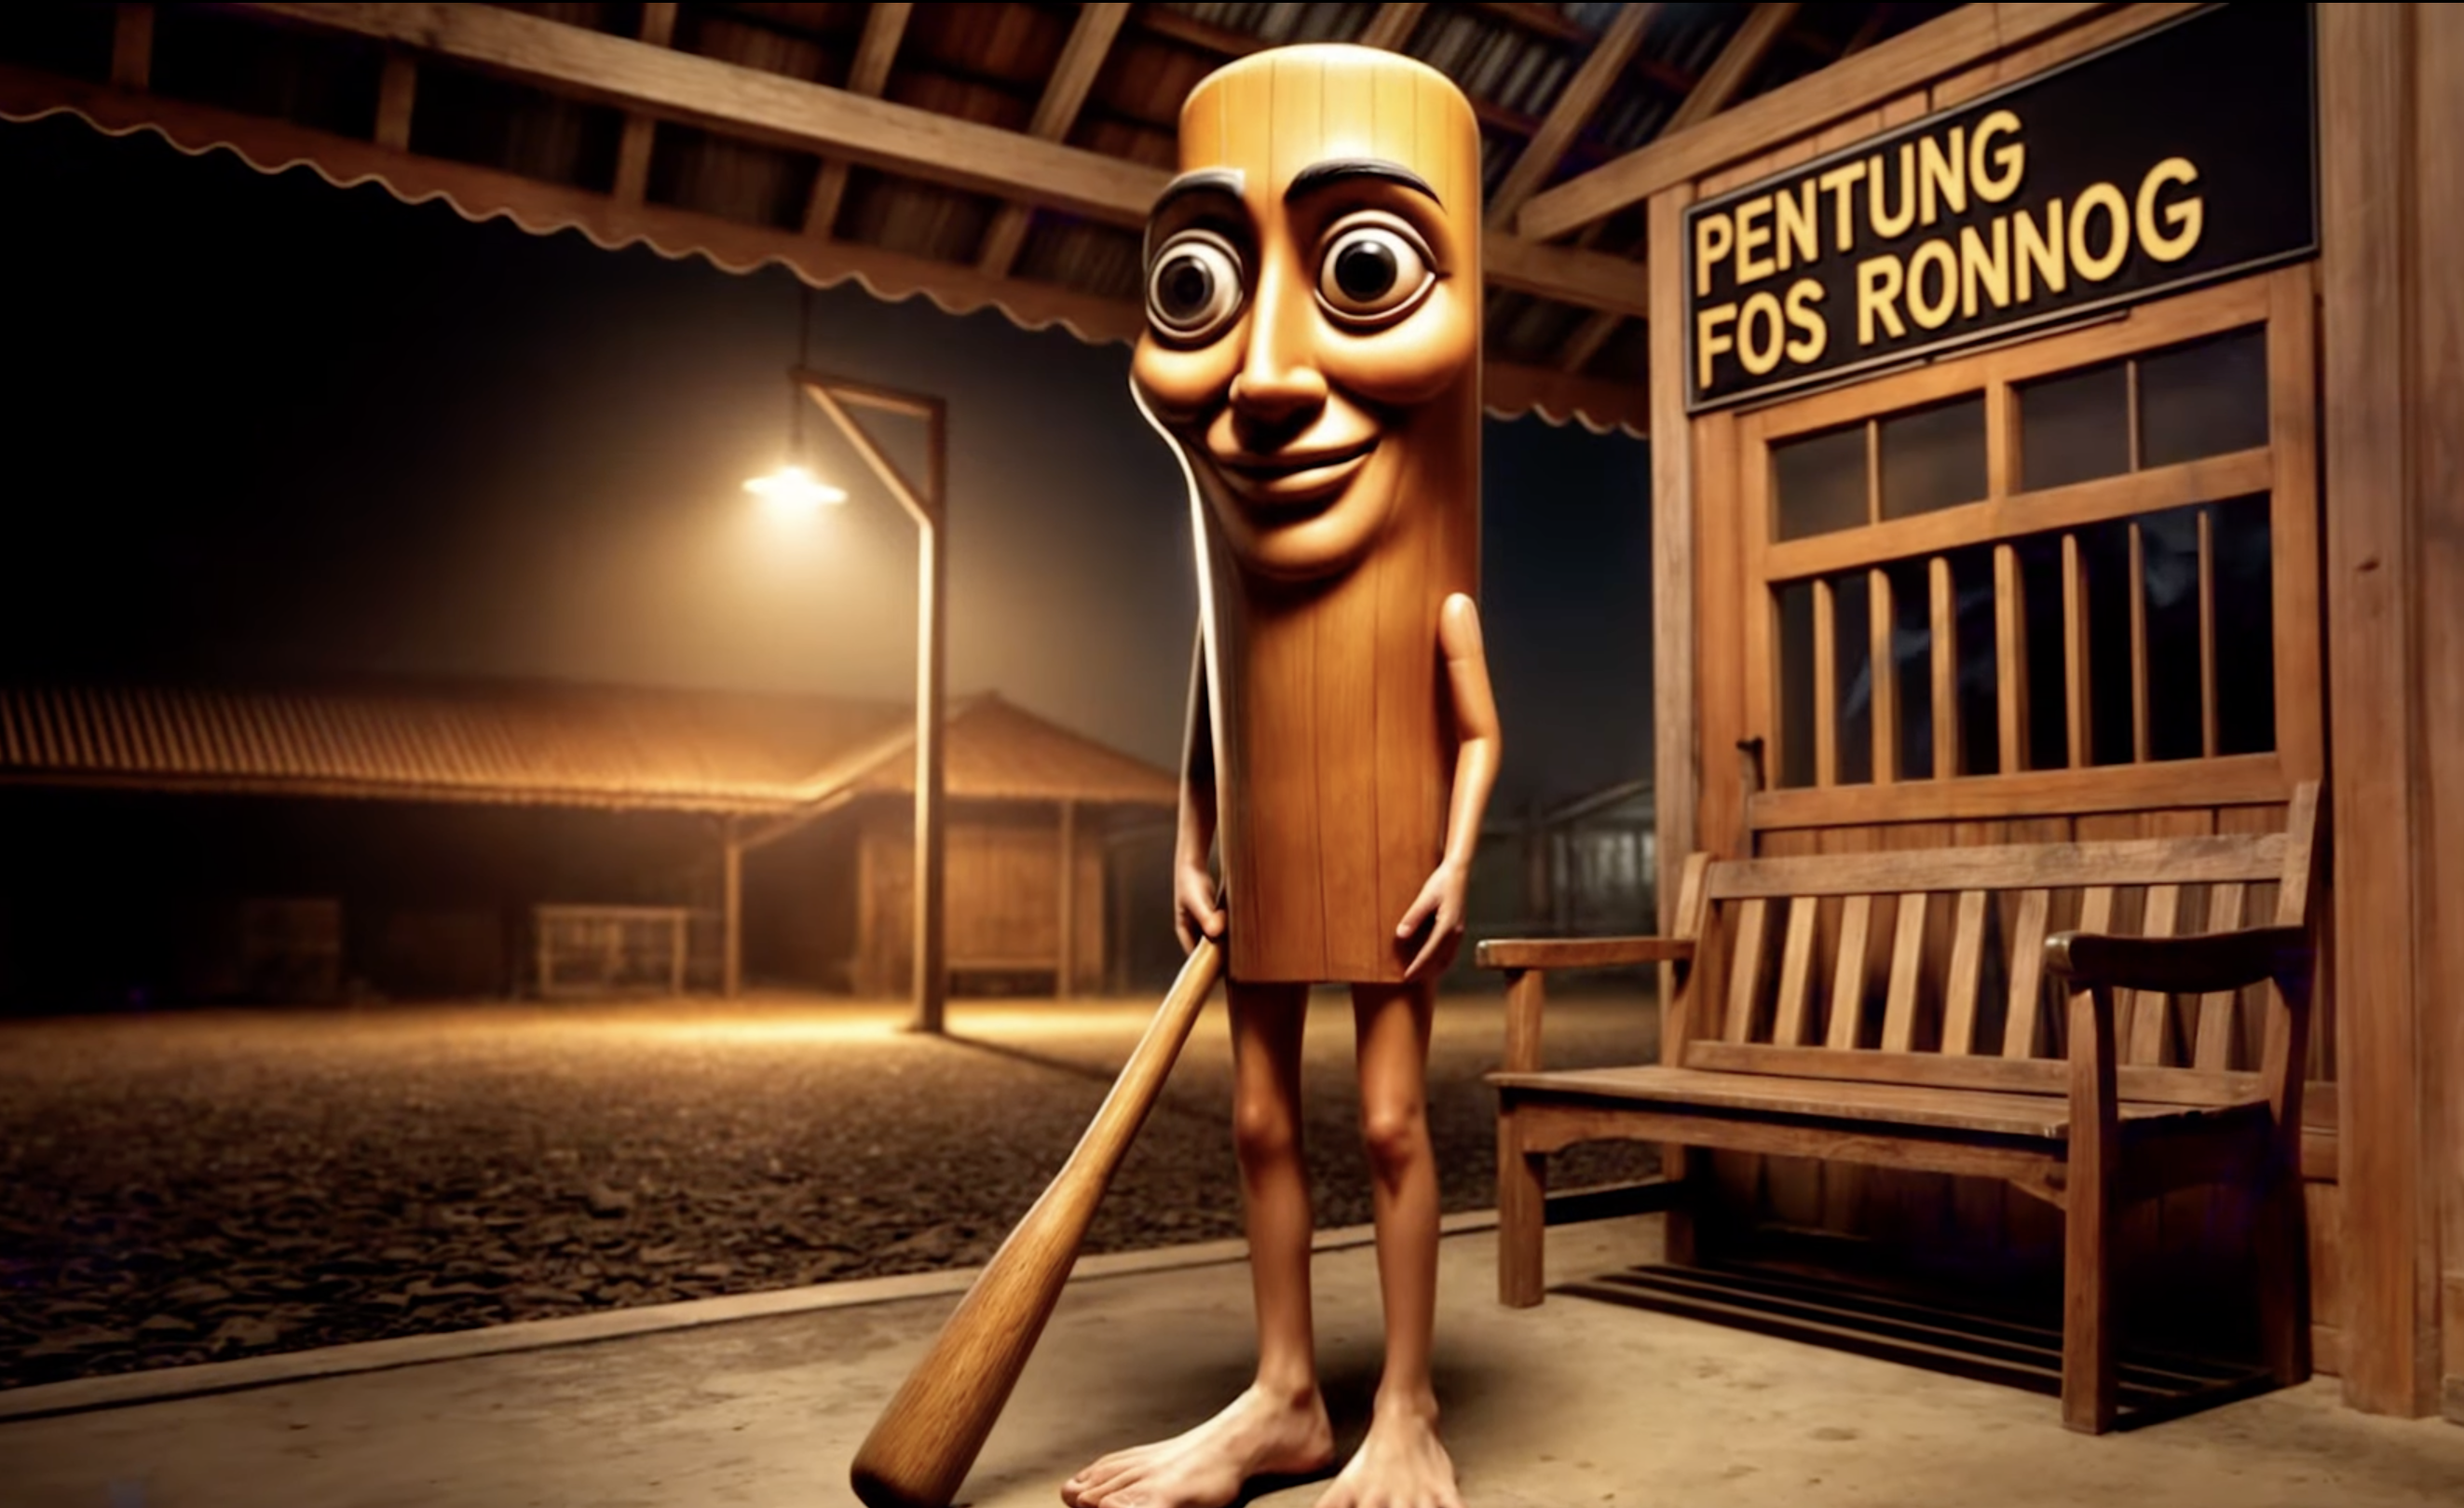
\includegraphics[scale = 0.2]{tungtungtunsahur.png}}
    \caption{Tung Tung Tung Sahur \href{https://www.youtube.com/watch?v=HmIMmFAV4BY}{\url{https://www.youtube.com/watch?v=HmIMmFAV4BY}}}
  \end{figure}

  \begin{solution}
    % Enter your solution here.
  \end{solution}

  \question In this problem we will prove/disprove some basic results regarding existence of cycles and paths in a graph.
  \begin{parts}
    \part Prove or disprove that a forest with $n$ vertices and $m$ components will always have $n-m$ edges. 
    \begin{solution}
      % Enter your solution here.
    \end{solution}

    \part Prove or disprove that every $n$-vertex graph with at least $n$ edges contains a cycle.
    \begin{solution}
       % Enter your solution here.
    \end{solution}

    \part Prove that every graph $G$ contains a path of length atleast $\delta(G)$ where $\delta(G)$ represented the smallest degree of a vertex in $G$.
    \begin{solution}
      % Enter your solution here.
    \end{solution}

    \part Prove that every graph $G$ with $\delta(G) \geq 2$ contains a cycle of length at least $\delta(G)+1$, where $\delta(G)$ represented the smallest degree of a vertex in $G$.
    \begin{solution}
      % Enter your solution here.
    \end{solution}
  \end{parts}

  \question In this problem we will see how a lot of our theorems and intuition breaks when it comes to infinite graph. An infinite graph is a graph where the set the vertices is an infinite set. 
  \begin{parts}
      \part Show that if $G$ is a finite graph such that every vertex of $G$ has a degree of 2 then $G$ contains a cycle.
      \begin{solution}
          % Enter your solution here.
      \end{solution}

      \part Show that this isn't necessarily true if $G$ is an infinite graph.
      \begin{solution}
          % Enter your solution here.
      \end{solution}
      \part Construct an infinite graph $G$ such that every vertex of $G$ has a degree of 2 and $G$ contains a cycle.
      \begin{solution}
        % Enter your solution here.
      \end{solution}
  \end{parts}

  \question With some stroke of luck you finally were able to take some time out of your Habib schedule and manage to make it to an Eid dawat. There were $n$ people at the dawat no two people are of the same age. After 4 years of missing every event due to some assignment being due, you were shocked to see people giving each other Eidi. But sadly discrete maths made a permanent damage to your brain, instead of enjoying the event you were wondering how many times Eidi was given. You notices that every one gave Eidi to everyone who is younger than them but didn't gave it to anyone older than them. How many times Eidi was given? Find a closed form formula in terms of $n$ and given a formal proof for your answer.
  \begin{solution}
    % Enter your solution here.
  \end{solution}

  \question The gates of the digital world are open. You are part of the DigiDestined who entered the digital world. As soon as you and the other DigiDestined enters the digital world you are all greeted with a bunch rookie digimons. Following the path of all the previous DigiDestines you will all partner up with one of those digimons and fight the forces of evil to save the digital world and the real world. But the tricky part is partnering with the digimons. Talking with the DigiDestines and the digimons you find out that every DigiDestined likes exactly $n$ digimons, and every digimon likes exactly $n$ DigiDestines, for some positive integer $n$. Can you pair every DigiDestined with a digimon such that everyone either gets a digimon they like or a digimon that likes them (no two people gets the same digimon)? Give a formal proof for your answer.
  \begin{figure}[h!]
    \centerline{
\includegraphics[scale = 0.075]{digimonadventure.png}}
    \caption{Original DigiDestined and their partner Digimons \href{https://www.imdb.com/title/tt9507234/}{\url{https://www.imdb.com/title/tt9507234/}}}
  \end{figure}
  \begin{solution}
    % Enter your solution here.
  \end{solution}
  
   
   

\end{questions}


\end{document}

%%% Local Variables:
%%% mode: latex
%%% TeX-master: t
%%% End:
